\section{Обзор предметной области}
\label{}

\subsection{Стандарт OpenGIS}
\label{}

GML (Geography Markup Language) является спецификацией OpenGIS® Implementation, в которой определяется кодировка XML для передачи и хранения географической информации. Спецификация опубликована на веб-сайте Открытого геопространственного консорциума (OGS).\\

\begin{figure}[h]
    \centering
    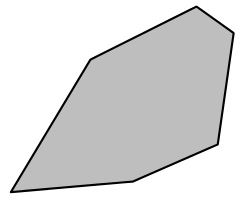
\includegraphics[width=0.33\textwidth]{gml.png}
    \caption{Пример кодирования многоугольника при помощи GML-разметки}
\end{figure}
\begin{lstlisting}[tabsize=2,breaklines,frame=single]{language=XML}
<gml:Polygon gml:id="p3" srsName="urn:ogc:def:crs:EPSG:6.6:4326">
	<gml:exterior>
		<gml:LinearRing>
			<gml:coordinates>5,5 28,7 44,14 47,35 40,40 20,30 5,5</gml:coordinates>
		</gml:LinearRing>
	</gml:exterior>
</gml:Polygon>
\end{lstlisting}

Open Geospatial Consortium (OGC) — международная некоммерческая организация, ведущая деятельность по разработке стандартов в сфере геопространственных данных и сервисов, созданная в 1994 году. В настоящее время координирует деятельность более 500 \cite{noauthor_open_nodate} правительственных, коммерческих, некоммерческих и научно-исследовательских организаций с целью разработки и внедрения консенсусных решений в области открытых стандартов для геопространственных данных, обработки данных геоинформационных систем и совместного использования данных. Большинство стандартов OGC основано на принципах, изложенных в базовой модели данных для представления географических характеристик под названием Abstract Specification. На основе базовой модели участники консорциума разработали и продолжают разрабатывать большое число спецификаций или стандартов для обслуживания конкретных потребностей организаций-участников в области геопространственных технологий и сервисов, включая ГИС.

Проект OpenGIS был инициирован до учреждения OGS, и впоследствии стал торговым знаком для ряда спецификаций, разрабатываемых и поддерживаемых в рамках этого консорциума. Стандарт GML определяет спецификацию географического языка разметки на основе синтаксиса XML. Этот язык позволяет кодировать географическую информацию, которая включает, в частности, геометрические характеристики объектов, в форме XML-документов. Такие документы могут использоваться для обмена геоданными между различными приложениями, обеспечивая их унификацию; для хранения геоданных и доступа к ним, в том числе и в среде глобальной сети; для публикации их на веб-сайтах. Разработка начальной версии языка GML (GML 1.0) была завершена весной 2000 года. Действующая в настоящее время версия этого стандарта - GML 3.3. Версия GML 3.1.0 была представлена консорциумом OGC в ISO в 1994 г. для создания на ее основе официального международного стандарта, где в настоящее время  эта спецификация проходит принятую в ISO процедуру стандартизации \cite{noauthor_iso_nodate}.

\begin{figure}[h]
    \centering
    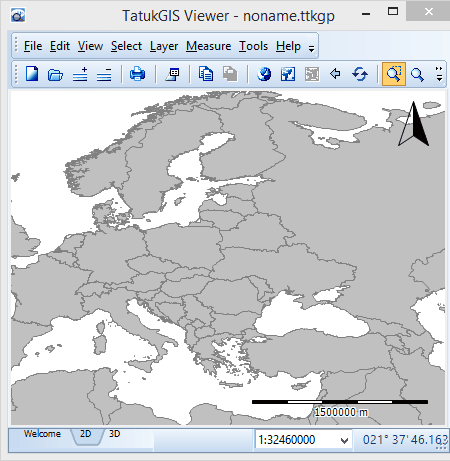
\includegraphics{tatuk.png}
    \caption{Интерфейс программы TatukGIS Viewer}
\end{figure}

Для работы с данными, закодированными в GML и сходных стандартах, компанией TatukGIS была разработана соответствующая линейка приложений. В частности, для визуализации данных в данной работе использовался TatukGIS Viewer.

\subsection{Существующие решения}
\label{}

Большинство алгоритмов упрощения топологии ГИС-файлов предназначаются для количественных преобразований (уменьшение размера файла), а не качественных. Однако, подобные задачи возникают в теории дифференциальных уравнений в частных производных и теории функций комплексной переменной --- в частности, при доказательстве интегральной теоремы Коши для многосвязной области \cite{__nodate}; а также в теории дифференциальных уравнений в частных производных --- например, при решении уравнения Лапласа в многосвязной области \cite{crowdy_transform_2015}.

\begin{figure}[h]
    \centering
    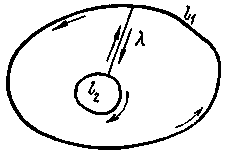
\includegraphics[width=0.4\textwidth]{koshi.png}
    \caption{Интегральная теорема Коши для многосвязной области}
\end{figure}

Задача \ref{task2}, а, точнее, ее предельный случай при $N=3$ (задача о триангуляции многоугольника \cite{de_berg_chapter_2000}), широко известна в области трехмерной графики, поскольку в ней треугольник является фундаментальной единицей для составления более сложных объектов. Однако, прямое использование алгоритма триангуляции для решения задачи \ref{task2} очень неэффективно.

\begin{figure}[h]
    \centering
    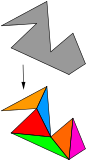
\includegraphics[width=0.2\textwidth]{triangulation.png}
    \caption{Задача о триангуляции многоугольника}
\end{figure}

\subsection{Теоретические сведения}
\label{}

\subsubsection{Топология}
\label{}

\textbf{Топология} --- раздел математики, занимающийся изучением свойств фигур (или пространств), которые сохраняются при непрерывных деформациях, таких, например, как растяжение, сжатие или изгибание. Непрерывная деформация – это деформация фигуры, при которой не происходит разрывов (т.е. нарушения целостности фигуры) или склеиваний (т.е. отождествления ее точек). Такие геометрические свойства связаны с положением, а не с формой или величиной фигуры.

Одной из характеристик фигур, инвариантных относительно непрерывных деформаций, является порядок связности. В \ref{task1} использовалось понятие односвязности. В простейшем двумерном случае односвязная фигура --- такая, в которой любой замкнутый путь можно непрерывно стянуть в точку. Проще говоря, это фигура, в которой отсутствуют <<дыры>>. Двусвязная область имеет одну дыру, трехсвязная – две, и т.д. При этом форма областей и дыр не имеет значения \cite{__2012}.

\begin{figure}[h]
    \centering
    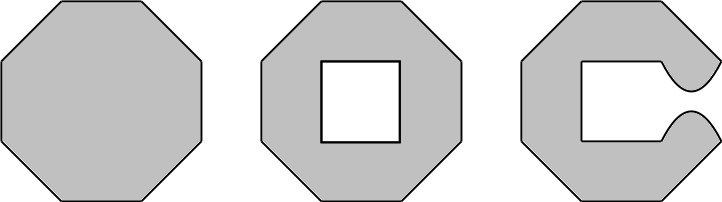
\includegraphics[width=1\textwidth]{topology.png}
    \caption{Слева направо: односвязная область, двусвязная область, преобразование двусвязной области в односвязную}
\end{figure}

Поскольку поставленная задача состоит в изменении порядка связности, конкретно --- в его уменьшении, она не может быть решена при помощи непрерывных деформаций. Требуется внести в многосвязные области разрезы при минимальном изменении их существенных характеристик. Эта цель достигается при помощи вырожденных туннелей: отрезок, по которому производится разрез, дважды вносится в границу результирующей области, благодаря чему площадь области не изменяется.

\begin{figure}[ht]
    \centering
    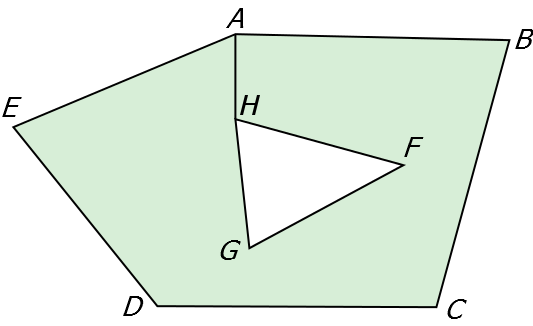
\includegraphics[width=0.7\textwidth]{reduce.png}
    \caption{Упрощение топологии полигональной области: $ABCDE \setminus FGH = ABCDEAHGFHA$}
    \label{fig:polysimp}
\end{figure}

\subsubsection{Теория графов}
\label{}

Для решения задачи \ref{task1} будет использован \textit{алгоритм Прима} из теории графов.

Граф – это совокупность двух множеств: множества точек, которые называются вершинами, и множества ребер А. Ребра --- это неупорядоченные (для неориентированного графа) или упорядоченные (для ориентированного) пары элементов из множества вершин, которые называются концами ребра. Если каждому ребру сопоставляется некоторое число (вес), то граф называется взвешенным. 

Дерево --- это граф, не имеющий циклов, т.е. замкнутых путей. Остов графа --- это его подграф, содержащий все вершины исходного, но являющийся деревом. Минимальный остов взвешенного графа --- это остовное дерево, имеющее наименьший суммарный вес ребер \cite{__2010}.

Алгоритм Прима используется для поиска в неориентированном взвешенном графе минимального остовного дерева. В нем искомый минимальный остов строится постепенно, путем добавлением в него ребер по одному. Изначально остов полагается состоящим из единственной вершины, взятой произвольно. Затем выбирается ребро минимального веса, исходящее из этой вершины, и добавляется в минимальный остов. Далее на каждом шаге ищется минимальное по весу ребро, один конец которого — уже взятая вершина, а другой — ещё не взятая, и это ребро добавляется в остов (если таких рёбер несколько, можно взять любое). Этот процесс повторяется до тех пор, пока остов не будет содержать все вершины \cite{prim_shortest_1957}. Без дополнительных оптимизаций алгоритм Прима работает за квадратичное время.

Альтернативой алгоритма Прима является алгоритм Краскала. В нем текущее множество ребер вначале устанавливается пустым. Затем, пока это возможно, проводится следующая операция: из всех рёбер, добавление которых к уже имеющемуся множеству не вызовет появление в нём цикла, выбирается ребро минимального веса и добавляется к уже имеющемуся множеству. Когда таких ребер больше нет, алгоритм завершён. Подграф данного графа, содержащий все его вершины и найденное множество рёбер, является его остовным деревом минимального веса \cite{kruskal_shortest_1956}.

Можно показать, что в пределе время выполнения алгоритма Прима пропорционально количеству вершин \cite{prim_shortest_1957}, а алгоритма Краскала --- количеству ребер \cite{kruskal_shortest_1956}. Поскольку в данной работе требуется искать минимальный остов в графах, близких к полным, то оптимально будет использование алгоритма Прима. Дополнительным преимуществом является простота реализации.